\documentclass[10pt,a4paper]{iace.report}
\usepackage[utf8]{inputenc}
\usepackage{ngerman}
\usepackage{graphicx}
\usepackage{amsmath}
\usepackage{amssymb}
\usepackage{amsfonts}
\usepackage{relsize}
\usepackage{media9} 
\usepackage{tikz}
\usepackage[overload]{empheq}
\usetikzlibrary{arrows, matrix, trees, mindmap, positioning}
\usepackage{arydshln}
\usepackage{animate}
\usepackage{anyfontsize}
\usepackage{bm}
\usepackage{wrapfig}
\newcommand{\tikzfnt}{13}

% Titlepage settings
\title{3DCSM - Body Handling\\\small Dynamische Modellierung und Entwurf eines Regelungskonzeptes}
\author{Bernd Heufelder}
\date{\today}

\begin{document}
	\maketitle
	\tableofcontents
	\newpage
	\chapter{Modellbildung und Parametrierung (AP 2)}
		\section{Dynamisches Modell des Body-Handlings (AP 2.1)}
			\subsection{Ziel des Arbeitspaketes}
				Das Ziel dieses Arbeitspaketes ist die Erstellung eines dynamischen Modells des Body-Handling-Systems. Besonders das Einschwingverhalten des Endeffektors und die Auswirkung verschiedener Trajektorien auf dieses Einschwingen ist von Interesse. Dafür wurden in diesem Arbeitspaket die folgenden Punkte umgesetzt:
				\begin{itemize}
					\item Abbildung des dynamischen Systemverhaltens, statische Aspekte stehen dabei im Hintergund
					\item Das Modell mit Abstraktion des Motors über Momentenvorgabe ist verfügbar
					\item Die um das Motormodell ergänzte Modellstruktur ist fertiggestellt
				\end{itemize}
			\subsection{Reduziertes mechanisches Modell}
				Das globale Koordinatensystem des Body-Handling Systems ist in Abbildung \ref{fig:cad} dargestellt. Der Aufbau besteht aus zwei Linearachsen in der yz-Ebene, zwei rotativen Achsen, der RotX-Achse und der RotBody-Achse. In Abbildung \ref{fig:cad} ist das 3D-Modell dieses Systems abgebildet. 
				\begin{figure}[h!]
					\centering
					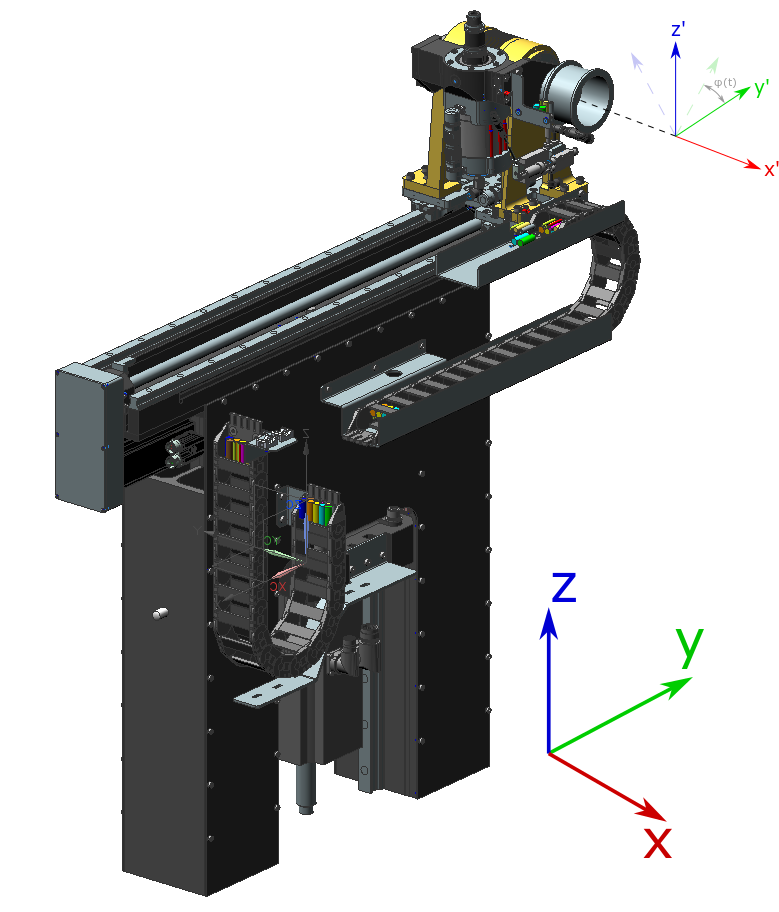
\includegraphics[width=0.6\linewidth]{./pics/aufbau_cad.png}
					\caption{CAD-Modell des Body-Handling-Systems}
					\label{fig:cad}
				\end{figure}
				Im schematischen Modell sind die beiden Linearachsen durch die Freiheitsgrade $ z(t),y(t) $ und die RotX-Achse durch den Freiheitsgrad $ \varphi(t) $ dargestellt. Die RotBody-Achse ist in diesem ebenen Modell nicht abgebildet, kann aber als eigenständiges System mit einem Freiheitsgrad behandelt werden. Die Vereinfachung auf ein ebenes Modell begründet sich daraus, dass dieses System kein Freiheitsgrad in x-Richtung aufweist. Im folgenden wird ausschließlich auf das Ebene Modell mit den Freiheitsgraden $ y,z $ und $ \varphi $ (Rotation um X) eingegangen. Dieses reduzierte Modell, mit den wichtigsten charakteristischen Federsteifigkeiten, ist in Abbildung \ref{fig:scematic} dargestellt.
				\begin{figure}[h!]
					\centering
					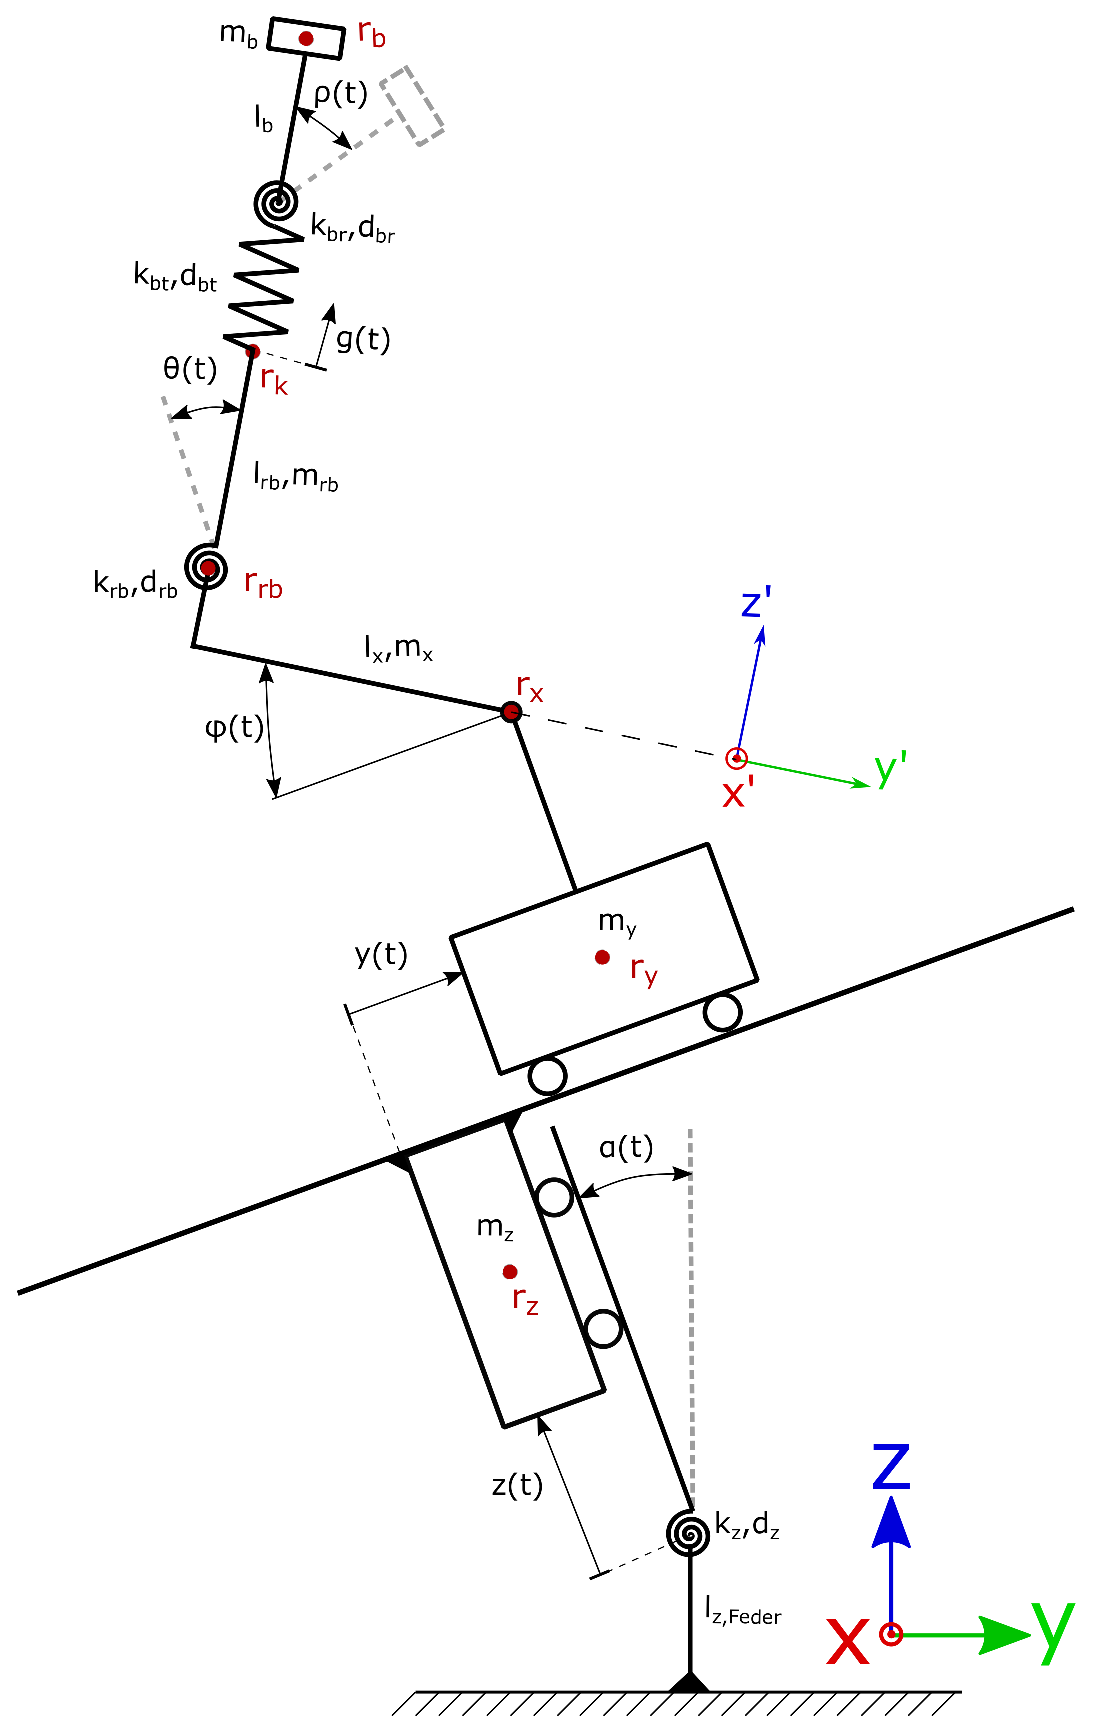
\includegraphics[width=0.78\linewidth]{./pics/SchematischesModell.eps}
					\caption{Schematisches reduziertes Modell}
					\label{fig:scematic}
				\end{figure}
				Die Auswahl der abgebildeten Federsteifigkeiten und die Begründung der vernachlässigten Steifigkeiten werden im Weiteren beschrieben. Welche Federsteifigkeiten relevant sind hängt davon ab ob das Systemverhalten im statischen oder im dynamischen Fall möglichst gut nachgebildet werden soll. Da das Ziel dieses Arbeitspaketes die Abbildung des dynamischen Systemverhaltens ist, wird der statische Aspekt bei der Auswahl der charackteristischen Federsteifigkeiten nicht berücksichtigt.
				 \subsubsection{Modellparameter}\label{sec:modellparameter}\leavevmode\\
					Die folgenden geometrische Parameter sind in  Meter angegeben:\\
					\vspace{10pt} \def\arraystretch{1.2}
					\begin{tabular}{lp{1cm}p{8.6cm}}
						$ l_{0x,z}=0.731 $ && \textit{Abstand in z-Richtung von der Feder des Unterbaus zur RotX-Achse für $ z=0 $}\\
						$ l_{0x,y}=0.119 $ &&\textit{Abstand in y-Richtung von der Feder des Unterbaus zur RotX-Achse für $ z=0$ } \\ 
						$ l_{z,Feder}=-0.11 $ &&\textit{Länge vom Ursprung zur Feder des Unterbaus} \\
						$ l_{x,y}=0.079 $ && \textit{Länge von der RotX-Achse ($ r_{x} $) zur RotBody Biegefeder ($ r_{rb} $) in y'-Richtung}\\
						$ l_{x,z}=0.039 $ && \textit{Länge von der RotX-Achse ($ r_{x} $) zur RotBody Biegefeder ($ r_{rb} $) in z'-Richtung}\\
						$ l_{rb}=0.06 $ &&\textit{Länge von der RotBody Biegefeder ($ r_{rb} $) zur Konusverbindung ($ r_{k} $)} \\
						$ l_{b}=0.0286 $ &&\textit{Länge von der Konusverbindung ($ r_{w} $) zum Schwerpunkt des Bodies ($ r_{b} $)}\\
					\end{tabular}\leavevmode\\
					Die Längen $ l_{x,y} $ und $ l_{x,z} $ sind auf das durch den Winkel $ \varphi $ mitgeführte Koordinatensystem bezogen.\\\\
					Die Massen der einzelnen Systembaugruppen sind in $ kg $ angeführt:\\\vspace{10pt} \def\arraystretch{1.2}
					\begin{tabular}{lp{1cm}p{8.6cm}}
						$ m_{y}=7.39 $ && \textit{Masse des y-Schlittens}\\ 
						$ m_{x}=4.87 $ && \textit{Masse der RotX-Armes, auf welchem die RotBody-Achse gelagert ist}\\ 
						$ m_{rb}=1.15 $ && \textit{Masse der RotBody-Achse}\\ 
						$ m_{b}=0.024 $ && \textit{Masse des Bodyholders inklusive der Masse des Bodies (Bestückobjekt)}\\ 
						$ m_{z} = 77.3 $ && \textit{Masse des Unterbaus}\\
					\end{tabular}\leavevmode\\
					Folgende Massenträgheitsmomente sind um X-Achse und den Schwerpunkt der jeweiligen Baugruppe in $ kgm^{2} $ angegeben: \\\vspace{10pt} \def\arraystretch{1.2}
					\begin{tabular}{lll}
						$ J_{x}=0.0126 $ & $ J_{rb}=0.0138 $ & $ J_{y} = 0.063 $ \\ 
						$ J_{b}=0.0000077 $  & $ J_{z}=7.191 $&  \\
					\end{tabular}\leavevmode\\
					Die wichtigsten Federkonstanten aus der Abbildung \ref{fig:scematic} sind im folgenden aufgelistet: \\\vspace{10pt} \def\arraystretch{1.3}
					\begin{tabular}{ll}
						$ k_{rb}=217.19\frac{kNm}{rad} $ & $ k_{br}=34.9\frac{kNm}{rad} $ \\ 
						$ k_{bt}=6069\frac{kN}{m} $ & $ k_{z}=2902.4\frac{kNm}{rad} $ \\   
					\end{tabular}\leavevmode\\
				In den folgenden Abschnitten werden die Federsteifigkeiten aus Abbildung \ref{fig:scematic} im Einzelnen betrachtet und deren Relevanz für das statische bzw. dynamische Systemverhalten bewertet. Die verwendeten Federsteifigkeiten wurden aus einem FEM-Modell von Swarovski bestimmt.
				 \subsubsection{Steifigkeit des Bodyholders (Konusverbindung)}\leavevmode\\
					\begin{align*}
					k_{Mx} &= 34.9\frac{kNm}{rad},\quad F_{ext}=20N,\quad l=0.075m,\quad r=0.0286m\\
					k_{Fz} &= 6069\frac{kN}{m}
					\end{align*}
					\begin{figure}[!h]
						\centering
						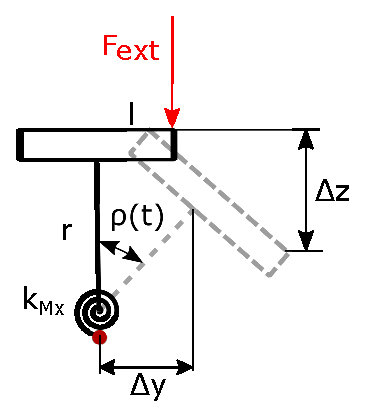
\includegraphics[width=0.3\linewidth]{./pics/bodyHolder.eps}\hspace{0.5cm}
						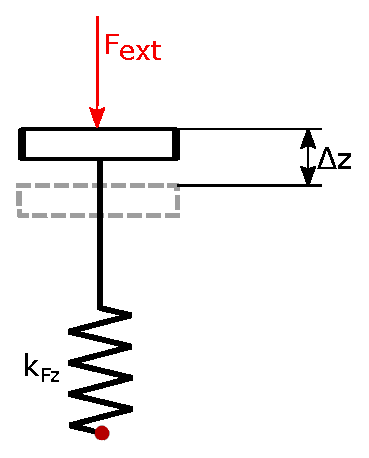
\includegraphics[width=0.25\linewidth]{./pics/bodyHolder_axial.eps}
					\end{figure}
					\begin{itemize}
						\item Rotative statische Auslenkung infolge einer externen Kraft\\
							\begin{align*}
							M_{ext} &= l\cdot F_{ext} = 1.5Nm,\\ 
							\Delta\rho &= \frac{M_{ext}}{k_{Mx}} = 42\mu rad\\
							\Delta z &= \Delta\rho\cdot l=\bm{3.15\mu m},\quad \Delta y=\Delta\rho\cdot r=\bm{1.20\mu m}
							\end{align*}
						\item Rotative dynamische Auslenkung infolge einer Beschleunigung mit 1g\\
							\begin{align*}
							M_g &=m_b\cdot g \cdot r =0.0067\text{Nm},\\ 
							\rho &= \frac{M_{g}}{k_{Mx}} = 0.193\mu rad\\
							\Delta y&=\rho\cdot r=\bm{0.55 \mu m}
							\end{align*}
						\item Rotative Eigenfrequenz mit leichtem Tool $  m_b=0.024kg $ \\
							\begin{align*} 
							f_{0} &= \bm{5687.2 Hz} 
							\end{align*}
						\item Axiale statische Auslenkung infolge einer externen Kraft\\
							\begin{align*}
							\Delta z &= \frac{F_{ext}}{k_{Fz}} = \bm{3.3\mu m}
							\end{align*}
						\item Axiale dynamische Auslenkung infolge einer Beschleunigung mit 1g\\
							\begin{align*}
							F_g &=m_b\cdot g = 0.235\text{N},\\
							\Delta z&=\frac{F_g}{k_{Fz}}= \bm{0.0387nm}
							\end{align*}
						\item Translatorische Eigenfrequenz mit leichtem Tool $  m_b=0.024kg $ \\
							\begin{align*}
							\bm{f_{0}} &= \bm{2515.4 Hz} 
							\end{align*}
					\end{itemize}
					Für die dynamische Betrachtung spielt die Steifigkeit der Konusverbindung eine vernachlässigbare Rolle. Durch die verhältnismäßig geringe modale Masse ergeben sich hohe Eigenfrequenzen im $ kHz $-Bereich. Als weitere Folge der geringen Masse entstehen auch nur vernachlässigbar kleine Auslenkungen.
					
                 \subsubsection{Biegesteifigkeit der Rot-Body-Achse}\leavevmode\\
	                \begin{align*}
	                	k_{Mx} &= 217.19\frac{kNm}{rad}, \quad F_{ext}=20N, \quad l=0.06m, \\ l_{com}&=0.05355m, \quad m_w=1.15kg
	                \end{align*}
	                \begin{figure}[!h]
	                	\centering
	                	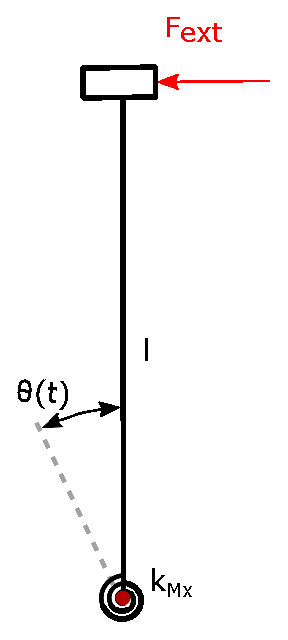
\includegraphics[width=0.2\linewidth]{./pics/rotBody.eps}
	                \end{figure}
	                \begin{itemize}
	                	\item Statische Auslenkung infolge einer externen Kraft\\
	                	\begin{align*}
	                	M_{ext} &= l\cdot F_{ext} = 1.2Nm,\\ 
	                	\Delta\theta &= \frac{M_{ext}}{k_{Mx}} = 5.525\mu rad\\
	                	\Delta y &= \theta\cdot l=\bm{0.33\mu m}      
	                	\end{align*}
	                	\item Dynamische Auslenkung infolge einer Beschleunigung von 1g
	                	\begin{align*}
	                	M_g &=m_w\cdot g \cdot l_{com}= 0.604 Nm\\ 
	                	\Delta\theta &= \frac{M_{g}}{k_{Mx}} = 2.78\mu rad\\
	                	\Delta y&=\Delta\theta\cdot l=\bm{0.17 \mu m}
	                	\end{align*}
	                	\item Eigenfrequenz ohne Bodyholder \\
	                	\begin{align*}
	                		f_{0} &= \bm{566.8 Hz}
	                	\end{align*}
	                \end{itemize}
                	Die translatorische Steifigkeit der RotBody-Achse wird nicht betrachtet, da die viel weichere Konusverbindung zum Bodyholder den größten Teil der Verformung verursacht. Auch die Steifigkeit der RotBody-Achse ist aufgrund der geringen Auslenkung und seiner Eigenfrequenz vernachlässigbar. 
                	
				 \subsubsection{Steifigkeit der RotX-Achse}\leavevmode\\
					\begin{align*}
						k_{Mx} &= 315\frac{kNm}{rad}, \quad F_{ext}=20N, \quad k_{Fy} = 57597\frac{kN}{m},\\ 
						l&=0.079m, \quad l_{com}=0.04534m, \quad m_x = 4.87kg
					\end{align*}
					\begin{figure}[!h]
						\centering
						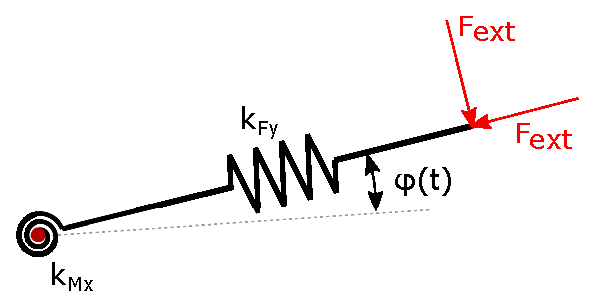
\includegraphics[width=0.4\linewidth]{./pics/rotX.eps}
					\end{figure}
					\begin{itemize}
						\item Rotative statische Auslenkung infolge einer externen Kraft\\
						\begin{align*}
						M_{ext} &= l\cdot F_{ext} = 1.58Nm\\
						\Delta\varphi &= \frac{M_{ext}}{k_{Mx}} = 5\mu rad\\
						\Delta z &= \Delta\varphi\cdot l=\bm{0.39\mu m}\\   
						\end{align*}
						\item Rotative dynamische Auslenkung infolge einer Beschleunigung von 1g
						\begin{align*}
						M_g &=m_x\cdot g \cdot l_{com}= 2.166Nm\\ 
						\Delta\varphi &= \frac{M_{g}}{k_{Mx}} = 6.87\mu rad\\
						\Delta z&=\Delta\varphi\cdot l=\bm{0.54 \mu m}
						\end{align*}
						\item Rotative Eigenfrequenz nur mit Masse $  m_{x} $  ohne $  m_{w}, m_{b} $ \\
						\begin{align*}
						f_{0} &= \bm{543.9 Hz} 
						\end{align*}
						\item Axiale statische Auslenkung infolge einer externen Kraft\\
						\begin{align*}
						\Delta y &= \frac{F_{ext}}{k_{Fy}} = \bm{0.35\mu m}\\ 
						\end{align*}
						\item Axiale dynamische Auslenkung infolge einer Beschleunigung von 1g
						\begin{align*}
						F_g &=m_x\cdot g = 47.77N\\ 
						\Delta y &= \frac{F_{g}}{k_{Fy}} =\bm{ 0.83\mu m}
						\end{align*}
						\item Axiale Eigenfrequenz nur mit Masse $  m_{x} $  ohne $  m_{w}, m_{b} $ \\
						\begin{align*}
						f_{0} &= \bm{547.34 Hz} 
						\end{align*}
					\end{itemize}
					Die Steifigkeit der RotX-Achse hat zwar geringfügig mehr Auswirkung auf das dynamische Verhalten als die Konusverbindung und die RotBody-Achse, ist aber ebenfalls vernachlässigbar. Denn die Eigenfrequenzen liegen im Bereich um $ 0.5kHz $, wobei zusätzlich die Auslenkung noch unter $ 1\mu m $ liegen.  
					
				 \subsubsection{Biegesteifigkeit des Unterbaus}\leavevmode\\
				 	\textbf{Ziel: } Federsteifigkeit des Unterbaus durch eine Biegefeder möglichst akkurat für alle Stellhöhen des Unterbaus anpassen.\\
				 	\textbf{Ausgangsdaten: } Aus der FEM-Simulation stehen 4 verschiedene Stellhöhen des Unterbaus (z-Höhe genannt) mit jeweils einer zugehörigen Eigenfrequenz zur Verfügung:
				 	\begin{itemize}
				 		\item Messung 1: $ z=0.5265m, \quad f_{0}=86Hz $
				 		\item Messung 2: $ z=0.6405m, \quad f_{0}=80Hz $
				 		\item Messung 3: $ z=0.7465m, \quad f_{0}=70Hz $
				 		\item Messung 4: $ z=0.8865m, \quad f_{0}=56Hz $
				 	\end{itemize}
				 	\textbf{Vorgehensweise: } Die Biegefeder wird in ihrer Federsteifigkeit und ihrer Positionierhöhe variiert um für alle z-Höhen möglichst genau die Eigenfrequenz aus der FEM-Simulation zu erhalten.					
					\begin{figure}[h!]
						\centering
						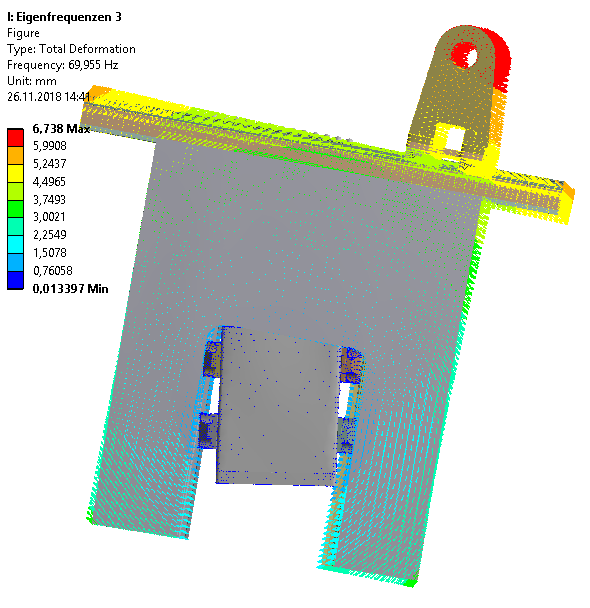
\includegraphics[width=0.40\linewidth]{./pics/fem_unterbau3.png}
						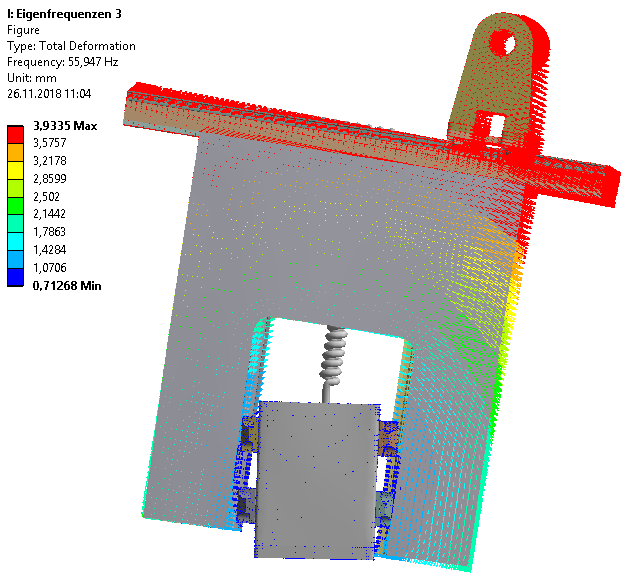
\includegraphics[width=0.45\linewidth]{./pics/fem_unterbau4.png}
						\caption{Beispielilustration der FEM-Simulationen}
					\end{figure}\leavevmode\\\\
					\textbf{Berechnung der gemittelten Federsteifigkeit}\\ 
					Die Abstände der Massenmittelpunkte des Unterbaus ($ MMP_{z} $) und des y-Schlittens ($ MMP_{y} $) zur Drehfeder des Unterbaus werden durch die Größen 
					\begin{align*}
						r_{z_{y}} &= l_{MMP_{y}}(z) - l_{z,Feder} \\
						r_{z_{z}} &= l_{MMP_{z}}(z) - l_{z,Feder}
					\end{align*}
					berechnet. Dabei sind $ l_{MMP_{y}}$ und $ l_{MMP_{z}} $ von der Höhe $ z(t) $ abhängigen Abstände vom Ursprung zu den Massenmittelpunkten in z-Richtung. Die Variable $ l_{z,Feder} $ ist die Positionierhöhe der Biegefeder.\\	
					Das resultierende Trägheitsmoment um die Biegefeder des Unterbaus ergibt sich mit den Trägheitsmomenten um die Schwerpunkte und dem Satz von Steiner zu
					\begin{align*}
						J_{Feder}(z) &= J_{y} + J_{z} + r_{z_{y}}^{2}(z)\cdot m_{y} + r_{z_{z}}^{2}(z)\cdot m_{z}.
					\end{align*}
					Die von der Höhe $ z $ abhängige Federsteifigkeit kann durch
					\begin{align*}
						k(z) &= \omega(z)^{2} \cdot J_{Feder}(z) 
					\end{align*}
					berechnet werden. Die Mittelwertbildung dieser Federsteifigkeit führt auf einen approximierten Wert. Der Fehler dieser gemittelten Steifigkeit wird minimiert, indem die Position $ l_{z,Feder} $ variiert wird. Ein Minimum erhält man für den Wert $  l_{z,Feder}=-0.11m $.\\\\
					Durch diese Berechnung ergibt sich eine mittlere Federsteifigkeit von $ k_{zr} = 2.9\cdot 10^{6} \frac{Nm}{rad} $ für die Biegefeder des Unterbaus. Eine Simulation mit dieser Federsteifigkeit zeigt, dass die Eigenfrequenzen bei verschiedenen Winkeln der RotX-Achse gut mit den Ergebnissen der FEM-Simulation übereinstimmen (siehe Abb. \ref{fig:nat_freq}).
					\begin{figure}
						\centering
						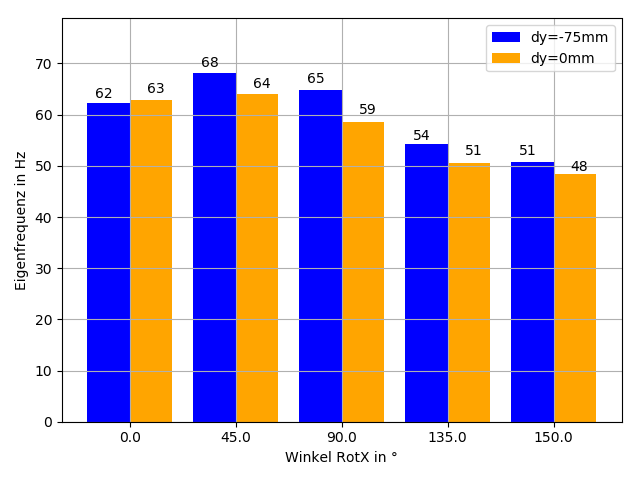
\includegraphics[width=0.49\linewidth]{./pics/eigenfreq_starr.png}
						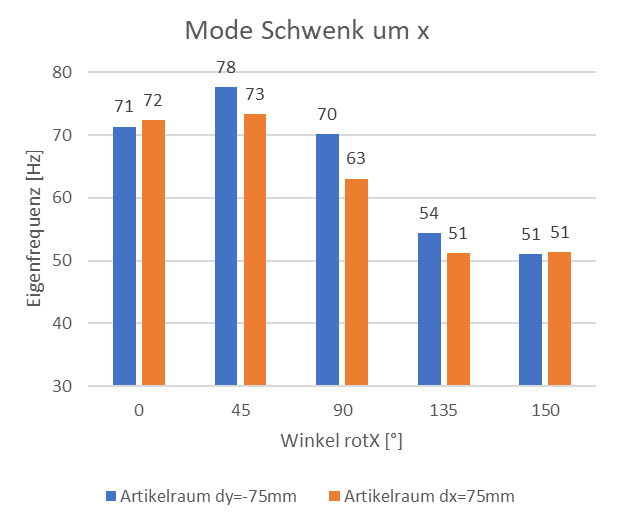
\includegraphics[width=0.49\linewidth]{./pics/eigenfreq_ref.png}
						\caption{links: Simulation des reduzierten Modells, rechts: FEM-Simulation}
						\label{fig:nat_freq}
					\end{figure}
					Durch den vertikalen Abstand von dieser Feder zum Bestückpunkt ergeben sich nicht vernachlässigbare Auslenkungen wie die folgende kurze Überschlagsrechnung zeigt. \\\\
					\textbf{Überschlagsrechnung: Auslenkung der Unterbaufeder durch eine Beschleunigung von $ 1g $}\\
					Das über die z-Höhe gemittelte Massenträgheitsmoment und der gemittelte vertikale Abstand von der Biegefeder zum Massenmittelpunkt des y-Schlittens werden aus den vier Messungen ermittelt und ergeben sich zu:
					\begin{align*}
						\bar{J}_{Feder} &= 14.8 kg\cdot m^{2}\\
						\bar{r}_{z_{y}} &= 0.6025 m.
					\end{align*}
					Die translatorische Beschleunigung von $ 1g $ kann durch den Abstand $ \bar{r}_{z_{y}} $ in eine Winkelbeschleunigung umgerechnet werden:	
					\begin{align*}
						\ddot{\alpha} = \frac{1\cdot g}{\bar{r}_{z_{y}}} &= 16.28\frac{rad}{s^{2}}.
					\end{align*}
					Das auf die Biegefeder wirkende Moment wird durch	
					\begin{align*}	
						M = \bar{J}_{Feder}\ddot{\alpha} &= 241Nm
					\end{align*}
					berechnet. Mit der gemittelten Federsteifigkeit kann die Winkelauslenkung bestimmt werden. Die Auslenkung des Endeffektors in y-Richtung ist durch $\Delta y$ dargestellt. 
					\begin{align*}	
						\alpha = \frac{M}{k_{zr}} &= 83.1 \mu rad\\ 
						\Delta y = \alpha\cdot l_{Feder-EE} &= 55.05 \mu m.
					\end{align*}
					Der Abstand $ l_{Feder-EE}=0.66m $ ist der Hebelarm von der Biegefeder zum Endeffektor. Da ein Versatz von $ 55.05 \mu m $ nicht vernachlässigbar ist, wird die Feder des Unterbaus im Modell berücksichtigt.
					
		\subsection{Herleitung der Bewegungsgleichungen}
			Um die erstellte Simulationsumgebung möglichst flexibel zu gestalten, werden die in den vorherigen Abschnitten als vernachlässigbar bezeichneten Federkonstanten mit ins Modell aufgenommen. Für eine Simulation ist es dadurch möglich einzelne Federn nach Belieben starr zu schalten. Mittels des Lagrange-Formalismus 2. Art werden die Zustandsdifferentialgleichungen aus der kinetischen und der potentiellen Energie hergeleitet. 
			\begin{align*}
			T_{t}&= \frac{1}{2}\bigg(m_{m}v_{com_{m}}^{2} +m_{d}v_{com_{d}}^{2}+m_{w}v_{com_{w}}^{2}+m_{b}v_{com_{b}}^{2}\bigg)\\  
			T_{r}&= \frac{1}{2}\bigg(J_{z}\dot{\alpha}^{2}+J_{x}(\dot{\alpha}+\dot{\varphi})^{2} +J_{w}(\dot{\alpha}+\dot{\varphi}+\dot{\theta})^{2} +J_{b}(\dot{\alpha}+\dot{\varphi}+\dot{\theta}+ \dot{\rho})^{2}\bigg)\\   
			U_{t} &= \frac{1}{2}k_{wt}g(t)^{2}\\
			U_{r} &= \frac{1}{2}\bigg(k_{z}\alpha(t)^{2}+ k_{rb}\theta(t)^{2}+k_{br}\rho(t)^2\bigg)\\
			\end{align*}
			Die Lagrange-Gleichung lautet
			\begin{equation*}
			L = T_{t}+T_{r} - (U_{t}+U_{r}).
			\end{equation*}
			Die zugehörigen Dissipationsfunktionen werden in einem separaten Term zusammengefasst:
			\begin{align*}
			D_{t} &= \frac{1}{2}d_{bt}\dot{g}(t)^{2}, \\
			D_{r} &= \frac{1}{2}\bigg(d_{z}\dot{\alpha}(t)^{2} + d_{rb}\dot{\theta}(t)^{2} + d_{br}\dot{\rho}(t)^{2}\bigg)\\
			D_{ges} &= D_{t} + D_{r}.
			\end{align*}
			Die extern auf das System einwirkenden Kräfte werden generalisierte Kräfte genannt und entsprechen den Kräften bzw. dem Moment, welche durch die elektrischen Antriebe ins System eingebracht werden.
			\begin{align*}
			Q & = [F_{y}, F_{z}, M_{\varphi},0 , 0, 0, 0]^{T}
			\end{align*}
			Damit lautet die Lagrange Gleichung 2. Art
			\[\frac{d}{dt}\bigg(\frac{\partial L}{\partial \dot{\bm{q}}} \bigg) -\frac{\partial L}{\partial \bm{q}} + \frac{\partial D_{ges}}{\partial \dot{\bm{q}}} = Q \]
			mit den zugehörigen Matrizen
			\begin{align*}
			M = \frac{\partial}{\partial\dot{\bm{q}}}\frac{\partial L}{\partial\dot{\bm{q}}}, \quad 
			C = \frac{\partial}{\partial\bm{q}}\frac{\partial L}{\partial\dot{\bm{q}}}, \quad
			F = \frac{\partial L}{\partial\bm{q}}, \quad 
			D = \frac{\partial D}{\partial\dot{\bm{q}}}.
			\end{align*}
			Durch Umformungen erhält man $ n $ Differentialgleichungen 2. Ordnung
			\[ M\ddot{\bm{q}} + C\dot{\bm{q}} - F = Q - D\]
			\begin{equation*}
			\Rightarrow \ddot{\bm{q}}=  M^{-1}(-C\dot{\bm{q}} + F + Q - D),
			\end{equation*}
			welche zur Simulation des Systems in $ 2\cdot n $ Differentialgleichungen 1. Ordnung umstrukturiert werden. 					
		
		\subsection{Vorwärtskinematik}
			Um die Position und Orientierung des Bestückpunktes zu bestimmen muss die Vorwärtskinematik für das System durchgeführt werden. Die Umrechnung auf den Bestückpunkt wird in die folgenden Transformationsmatrizen aufgeteilt: 
			\begin{align*}
			 T_{0-z,Feder} = &\begin{bmatrix}\cos\alpha(t) & -\sin\alpha(t) & 0\\\sin\alpha(t) & \cos\alpha(t) & l_{z,Feder}\\0&0&1 \end{bmatrix} , &\\
			 T_{z-x} = &\begin{bmatrix}-\cos\varphi(t) & \sin\varphi(t) & y(t)+l_{0x,y}\\\sin\varphi(t) & \cos\varphi(t) & z(t)+l_{0x,z}-l_{z,Feder}\\0&0&1 \end{bmatrix} , &\\
			 T_{x-rb} = &\begin{bmatrix}\cos\theta(t) & -\sin\theta(t) & l_{x,y}\\\sin\theta(t) & \cos\theta(t) & l_{x,z}\\0&0&1 \end{bmatrix}, &\\ 
			 T_{rb-b} = &\begin{bmatrix}\cos\rho(t) & -\sin\rho(t) & dy\\\sin\rho(t) & \cos\rho(t) & l_{w}+g(t)+l_{b}\\0&0&1 \end{bmatrix}& \\
			\end{align*}\leavevmode\\
			Die gesamt Transformationsmatrix ergibt sich schließlich durch Multiplikation dieser Matrizen zu
			\begin{align*}
				T_{0-b}&= T_{0-z,Feder}\cdot T_{z-x}\cdot T_{x-rb}\cdot T_{rb-b}.
			\end{align*}
			Ausgangspunkt ist der Ursprung $ \bm{r_{0}} = [0, 0]^{T} $, als homogene Koordinate $ \bm{r_{0}} = [0, 0, 1]^{T} $ wird dieser Punkt durch die Vorwärtskinematik auf den Bestückpunkt gemäß
			\begin{align*}
			\begin{bmatrix}\bm{r_{b}}\\1\end{bmatrix} = T_{0b}\cdot\begin{bmatrix}\bm{r_{0}}\\1\end{bmatrix}
			\end{align*}
			transformiert. Die Orientierung des Bestückpunktes ergibt sich als Summe der Einzelwinkel zu $ \psi(t) = \alpha(t)+\varphi(t)+\theta(t)+\rho(t) $.
			
		\subsection{Ergebnisse}
			In diesem Abschnitt wird eine Bewegung simuliert, welche eine Änderung der Bestückorientierung erfordert wobei die Bestückposition gleich bleiben soll. Die folgenden Randbedingungen gelten für alle in diesem Abschnitt beschriebenen Simulationen:
			\begin{itemize}
				\item Simulationszeit: $ t_{0} = 0, \quad T = 400ms $
				\item Bewegungsdauer: $ 200ms $
				\item Gewünschte Positonsverläufe der drei Achskoordinaten
				\begin{figure}[h!]
					\centering
					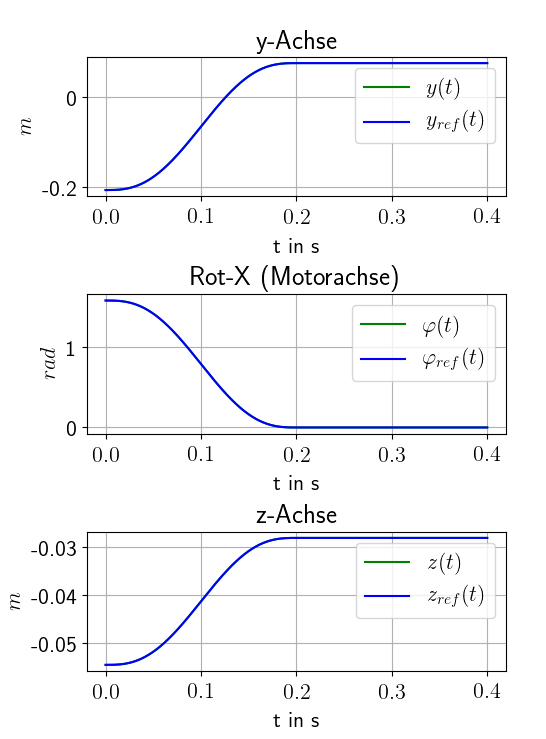
\includegraphics[width=0.5\linewidth]{./pics/inputs.png}
%					\caption{Eingangsgrößen der drei Achsen}
				\end{figure}
				\item Ausgangs- und Zielposition sind identisch. Die Orientierung der RotX-Achse wird jedoch geändert. Die Endeffektorposition und -orientierung wird zum Start- und Endzeitpunkt durch den Vektor
				\begin{align*}
				ee(t) &= [y_{ee}(t), z_{ee}(t), \psi(t)]\\
				ee(0) &= [0.04m,0.826m,90^{\circ}]\\
				ee(T) &= [0.04m,0.826m,0^{\circ}]
				\end{align*}	
				beschrieben.
				\item PID Regler für jede Achskoordinate (sehr steif ausgelegt)
				\item Regelung mit Vorsteuerung und computed torque
				\item Vorgabe Bestückposition und -orientierung für $ t_{0} $ und $ T $, Umrechnung und Bahnplanung in Gelenkskoordinaten
			\end{itemize}
			Es werden die nachfolgend aufgelisteten Simulationsstudien durchgeführt und miteinander verglichen:
			\begin{itemize}
				\item \textcolor{blue!60!black}{Simulation 1:} Starres System ($ \bm{q}=[y(t), z(t), \varphi(t)]^{T} $)
				\item \textcolor{blue!60!black}{Simulation 2:} Nur der Unterbau schwingt, restliches System ist starr ($ \bm{q}=[y(t), z(t), \varphi(t), \alpha(t)]^{T} $)
				\item \textcolor{blue!60!black}{Simulation 3:} Unterbau und RotBody-Achse sind schwingungsfähig ($ \bm{q}=[y(t), z(t), \varphi(t), \alpha(t), \theta(t)]^{T} $)
				\item \textcolor{blue!60!black}{Simulation 4:} Simulation 3 und zusätzlich Vorsteuerung mit Input-shaping	
			\end{itemize}
			
			 \subsubsection{\textcolor{blue!60!black}{Simulation 1:}}\leavevmode\\
				\begin{figure}[!h]
					\centering
					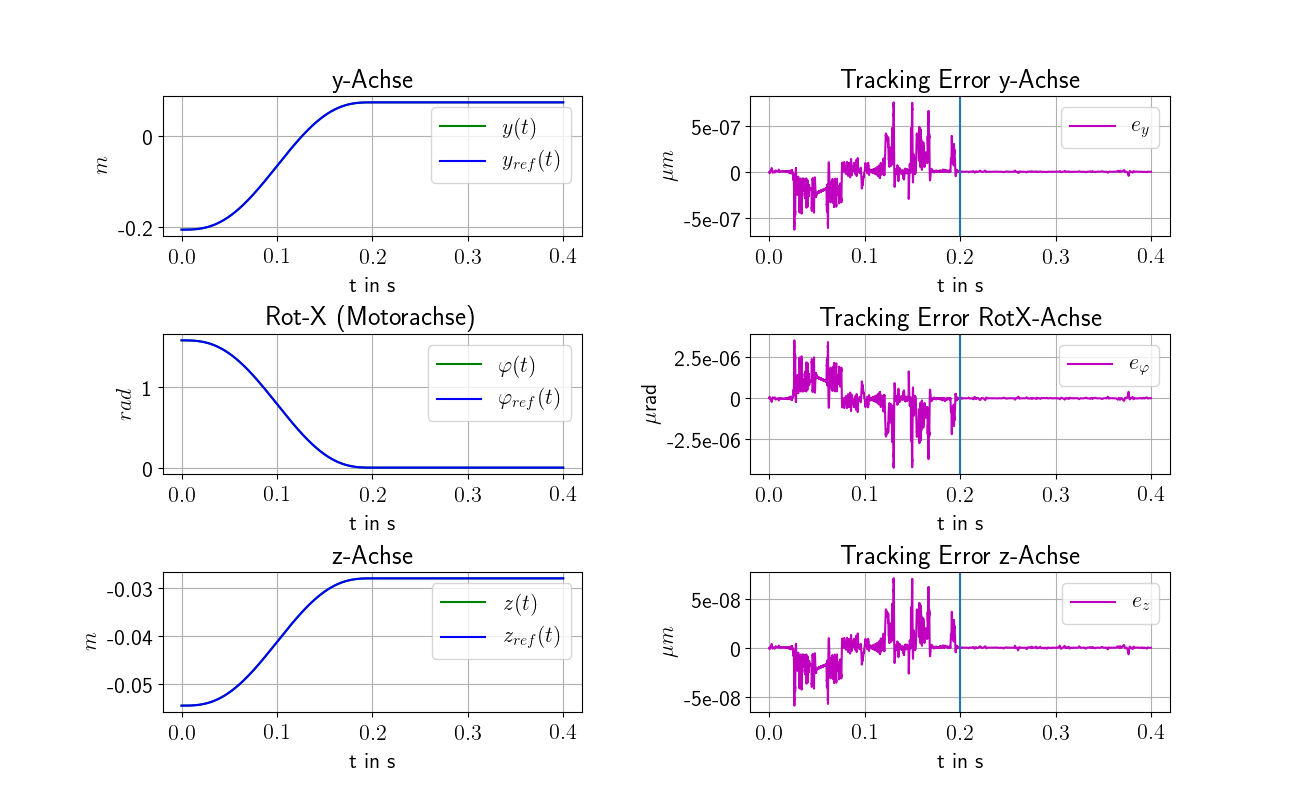
\includegraphics[width=0.99\linewidth]{./pics/posVerlaufAchsen_starr.png}
					\caption{Zeitlicher Verlauf der Achspositionen und deren Abweichung zu Referenztrajektorie}
					\label{fig:sim1pos}
				\end{figure}
				\begin{figure}[!h]
					\centering
					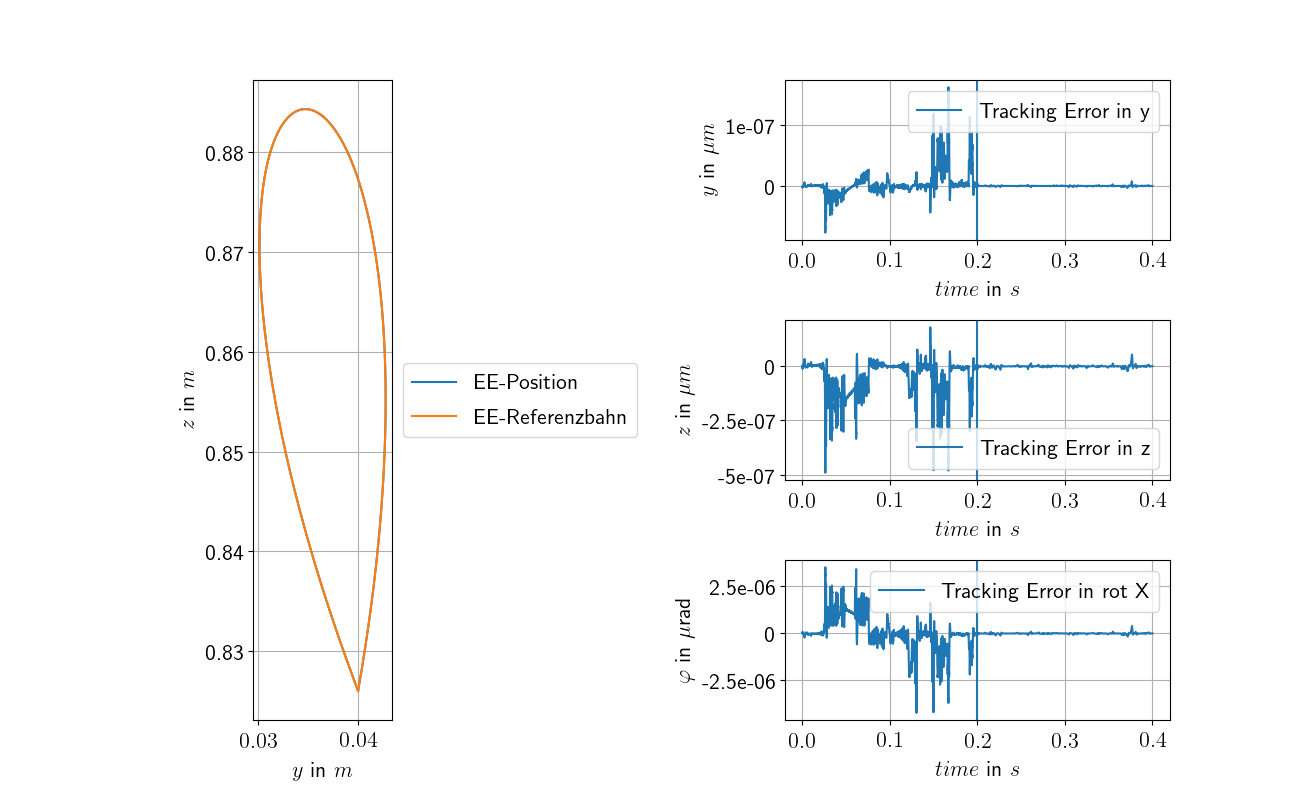
\includegraphics[width=0.99\linewidth]{./pics/endeffektor_starr.png}
					\caption{Endeffektorbahn in der yz-Ebene (links) und Tracking-Error der Endeffektorposition und -orientierung zur Referenzbahn}
					\label{fig:sim1ee}
				\end{figure}
				In der ersten Abbildung \ref{fig:sim1pos} ist zu sehen, dass die Achspositionen der geplanten Referenztrajektorie genau folgen. Der Tracking-Error der einzelnen Achsen ergibt sich aus numerischen Gründen und ist de facto nicht vorhanden. Die Bahn in der yz-Ebene ist in Abbildung \ref{fig:sim1ee} auf der linken Seite dargestellt. Rechts ist die Abweichung des Bestückpunktes von seiner Referenzbahn gezeigt.
				
			 \subsubsection{\textcolor{blue!60!black}{Simulation 2:}}\leavevmode
				\begin{figure}[!h]
					\centering
					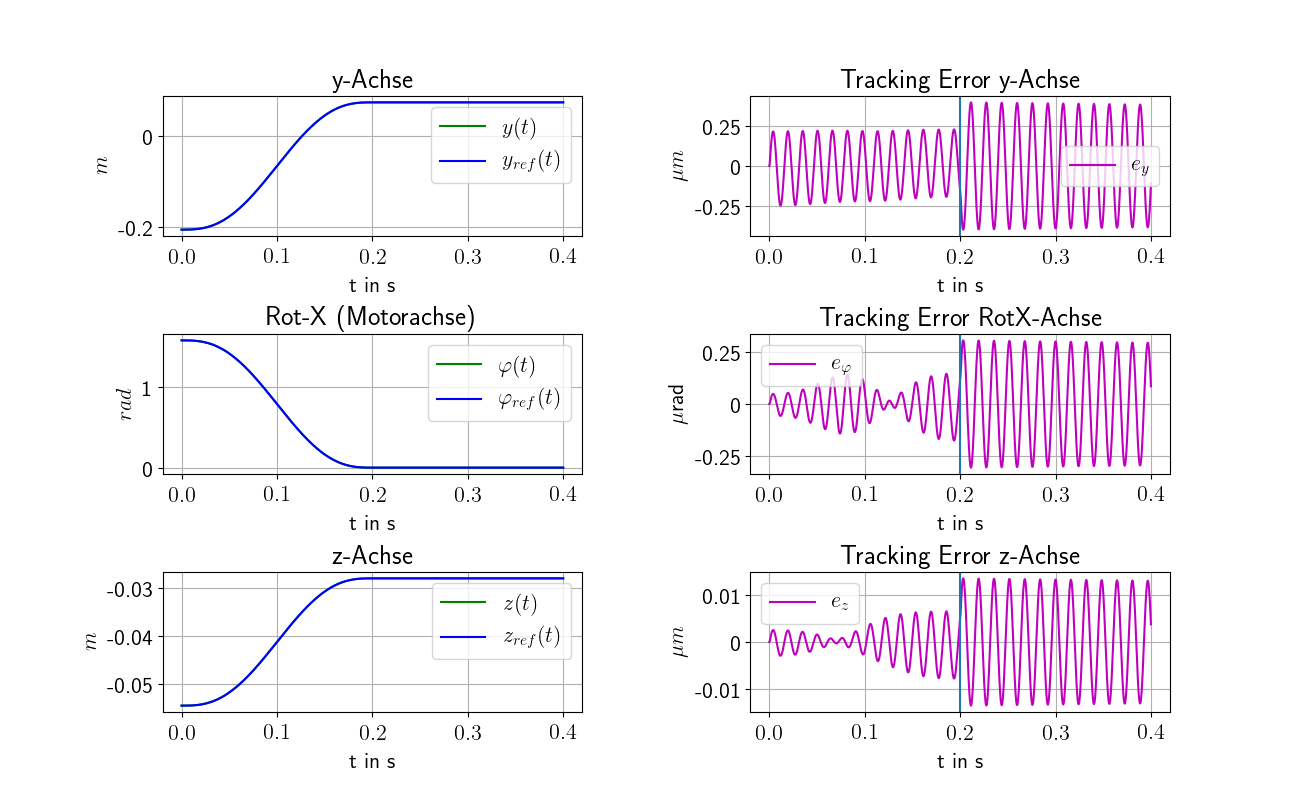
\includegraphics[width=0.99\linewidth]{./pics/posVerlaufAchsen_nurZ.png}
					\caption{Zeitlicher Verlauf der Achspositionen und deren Abweichung zu Referenztrajektorie}
					\label{fig:sim2pos}
				\end{figure}
				\begin{figure}[!h]
					\centering
					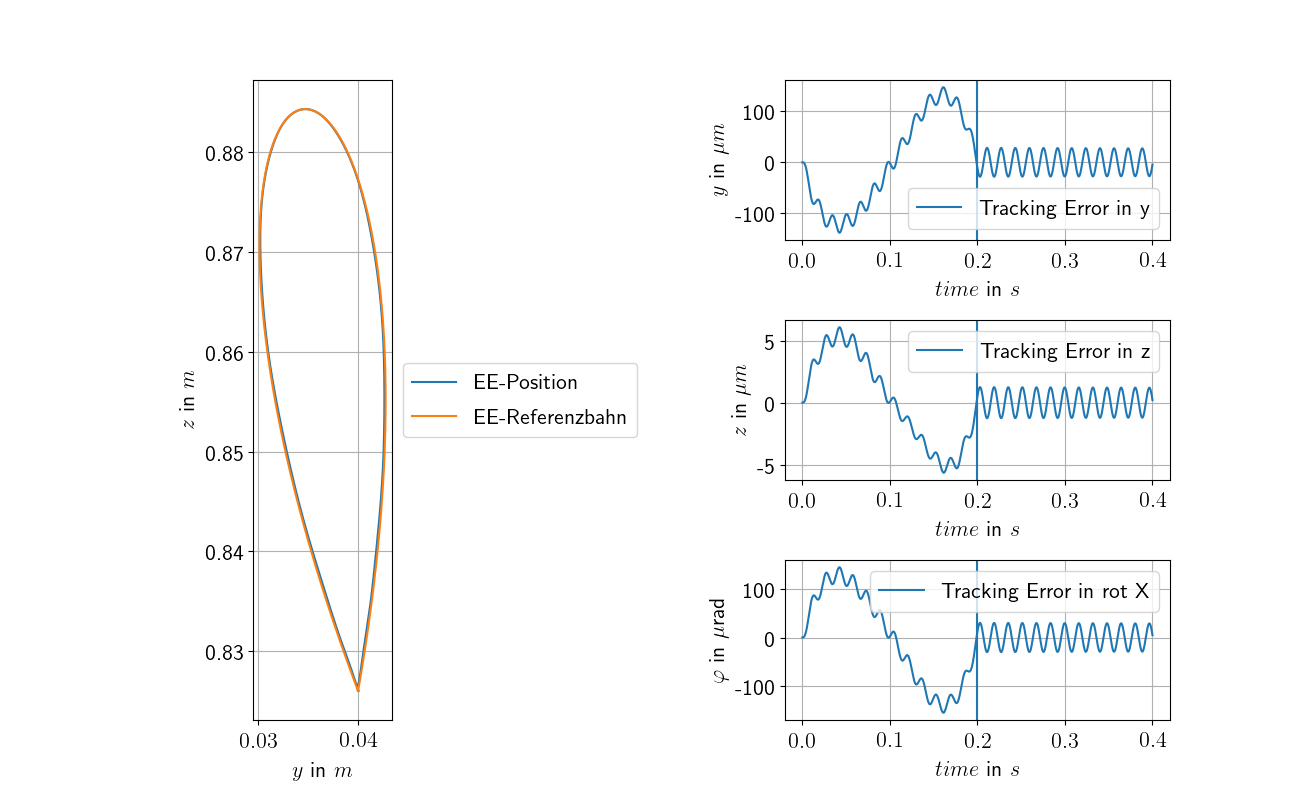
\includegraphics[width=0.99\linewidth]{./pics/endeffektor_nurZ.png}
					\caption{Endeffektorbahn in der yz-Ebene (links) und Tracking-Error der Endeffektorposition und -orientierung zur Referenzbahn}
					\label{fig:sim2ee}
				\end{figure}
				Mit zugeschalteter Unterbaufeder ist in Abbildung \ref{fig:sim2pos} und \ref{fig:sim2ee} ersichtlich, dass trotz geringer Abweichungen der einzelnen Achskoordinaten der Bestückpunkt deutlich mehr schwingt. Aus diesem Grund ist diese Biegefeder auch sehr wichtig für die dynamische Beschreibung des Systemverhaltens.
			 \subsubsection{\textcolor{blue!60!black}{Simulation 3:}}\leavevmode
				\begin{figure}[!h]
					\centering
					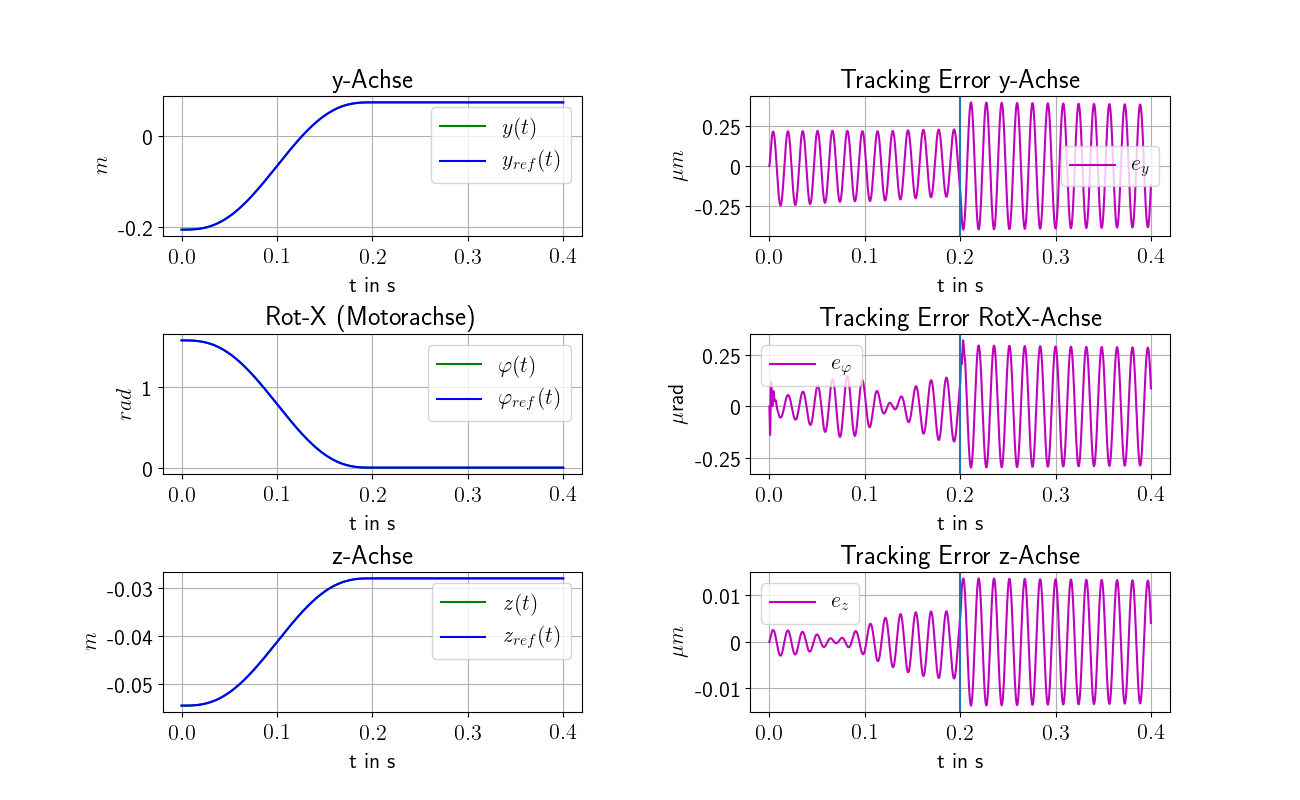
\includegraphics[width=0.99\linewidth]{./pics/posVerlaufAchsen_ZundTheta.png}
					\caption{Zeitlicher Verlauf der Achspositionen und deren Abweichung zu Referenztrajektorie}
					\label{fig:sim3pos}
				\end{figure}
				\begin{figure}[!h]
					\centering
					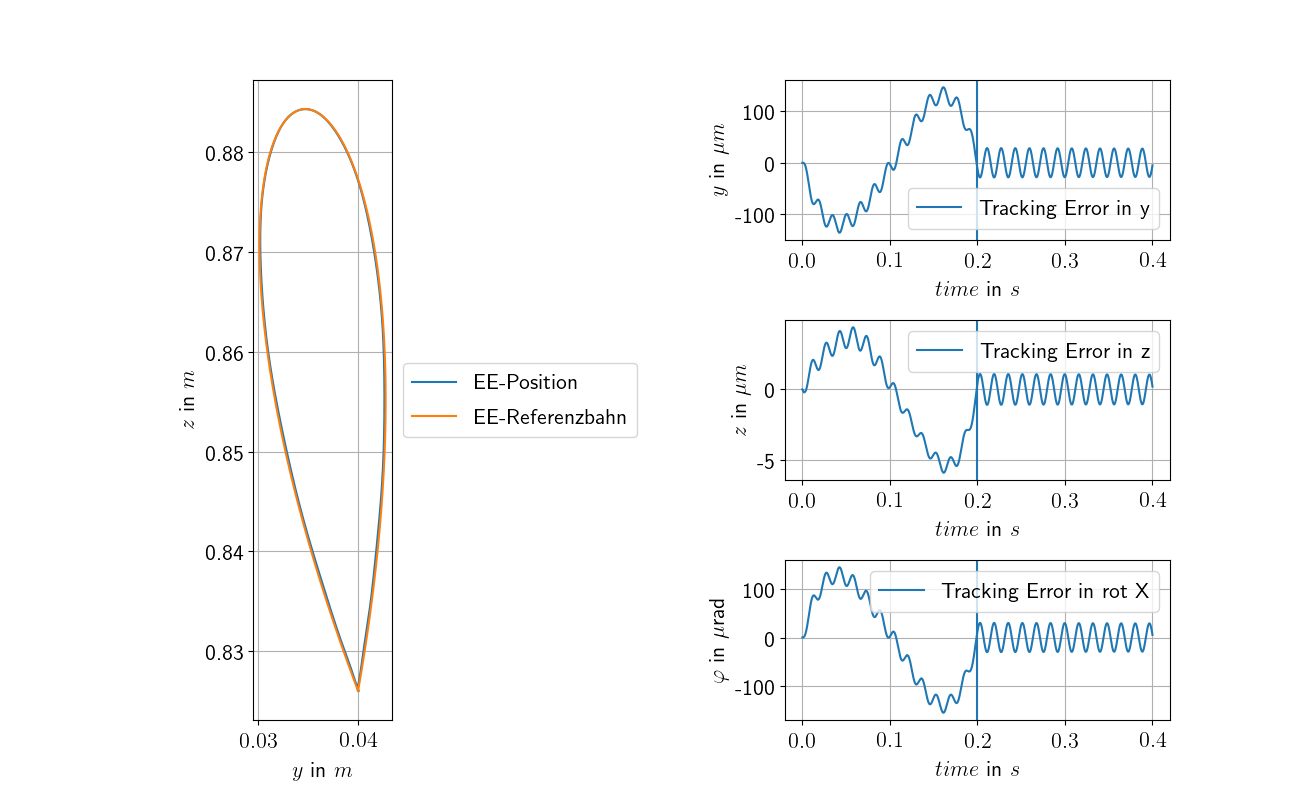
\includegraphics[width=0.99\linewidth]{./pics/endeffektor_ZundTheta.png}
					\caption{Endeffektorbahn in der yz-Ebene (links) und Tracking-Error der Endeffektorposition und -orientierung zur Referenzbahn}
					\label{fig:sim3ee}
				\end{figure}
				Aufgrund der geringeren Auslenkung der RotBody-Biegefeder (siehe Abb. \ref{fig:sim3federn}) in Kombination eines kürzeren Hebelarmes hat diese Feder eine vernachlässigbare Auswirkung auf die Bestückposition und -orientierung.
				\begin{figure}[!h]
					\centering
					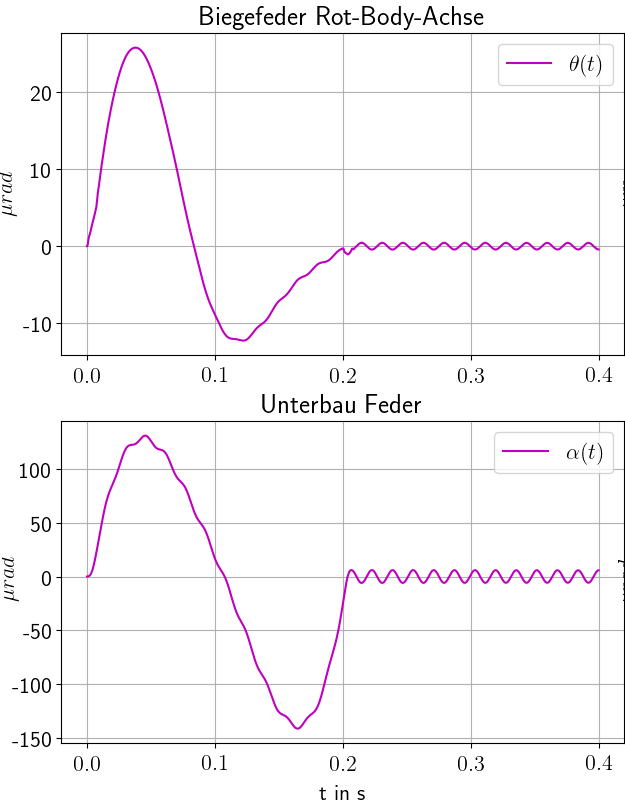
\includegraphics[width=0.6\linewidth]{./pics/federn_shift.png}
					\caption{Auslenkung der RotBody-Biegefeder (oben) und Auslenkung der Unterbau-Biegefeder (unten)}
					\label{fig:sim3federn}
				\end{figure}
			 \subsubsection{\textcolor{blue!60!black}{Simulation 4:}}\leavevmode
				\begin{figure}[!h]
					\centering
					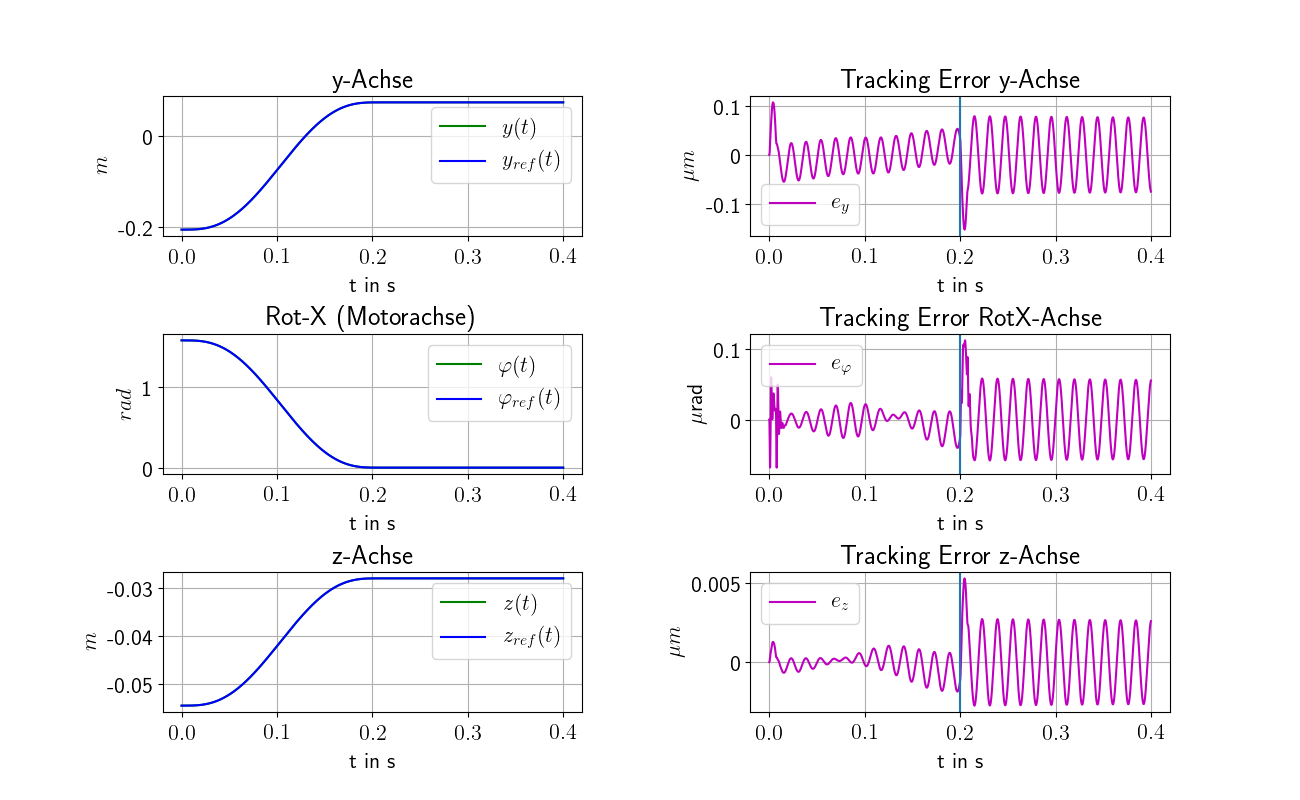
\includegraphics[width=0.99\linewidth]{./pics/posVerlaufAchsen_shift.png}
					\caption{Zeitlicher Verlauf der Achspositionen und deren Abweichung zu Referenztrajektorie}
					\label{fig:sim4pos}
				\end{figure}
				\begin{figure}[!h]
					\centering
					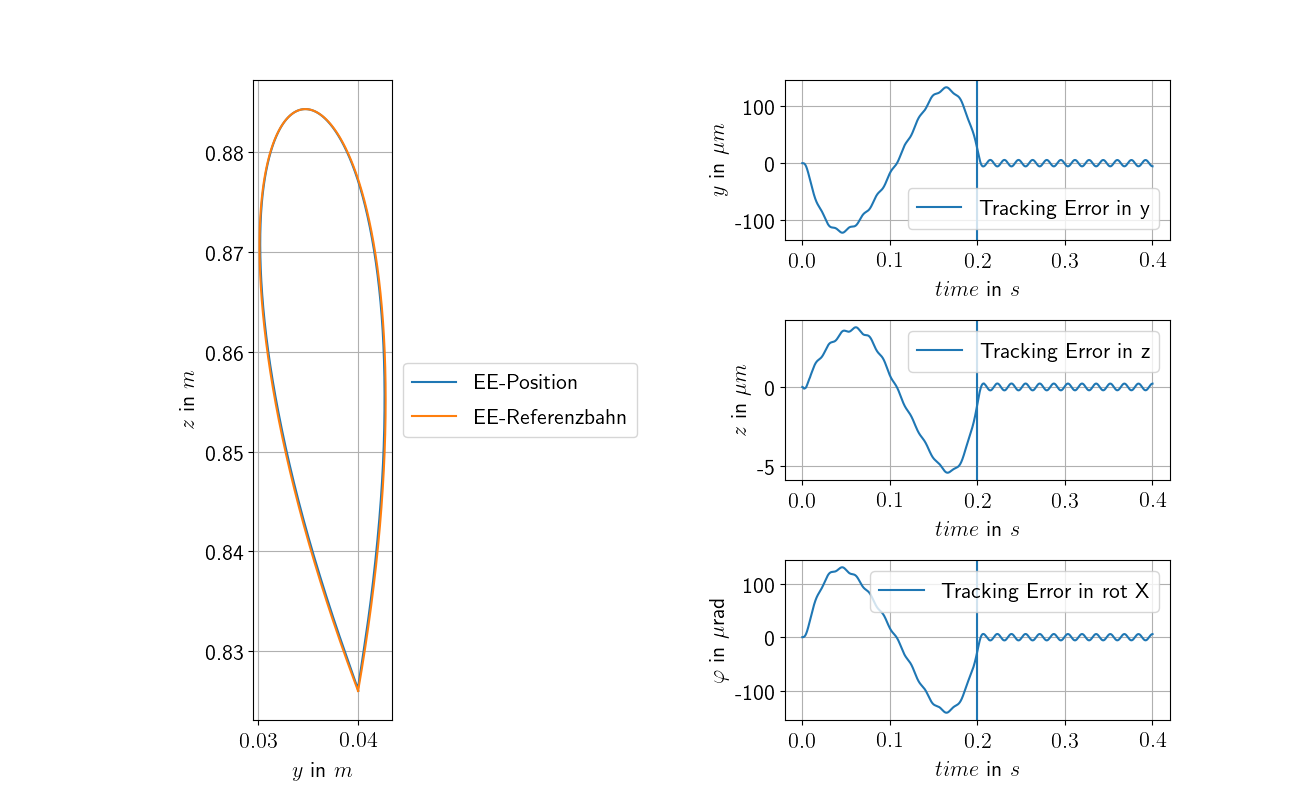
\includegraphics[width=0.99\linewidth]{./pics/endeffektor_shift.png}
					\caption{Endeffektorbahn in der yz-Ebene (links) und Tracking-Error der Endeffektorposition und -orientierung zur Referenzbahn}
					\label{fig:sim4ee}
				\end{figure}
				Mithilfe von \textit{Input-shaping} ist es anhand der Eigenfrequenzen des Systems möglich die Trajektorie so auszulegen, dass Eigenschwingungen, die zu Beginn der Bewegung angeregt werden, am Ende der Trajektorie kompensiert werden. In Abbildung \ref{fig:sim4ee} ist zu erkennen, dass sich damit die Amplitude der Schwingungen am Endeffektor etwa um den Faktor 20 reduzieren.
			\clearpage
		\subsection{RotX-Feder zur Eigengewichtskompensation}
			Zur Entlastung des Motors der RotX-Achse wurde, wie in Abb. \ref{fig:rotXspring} dargestellt, eine translatorische Feder ausgelegt um das Eigengewicht der an dieser Achse angehängten Massen zu kompensieren.
			\begin{figure}[!h]
				\centering
				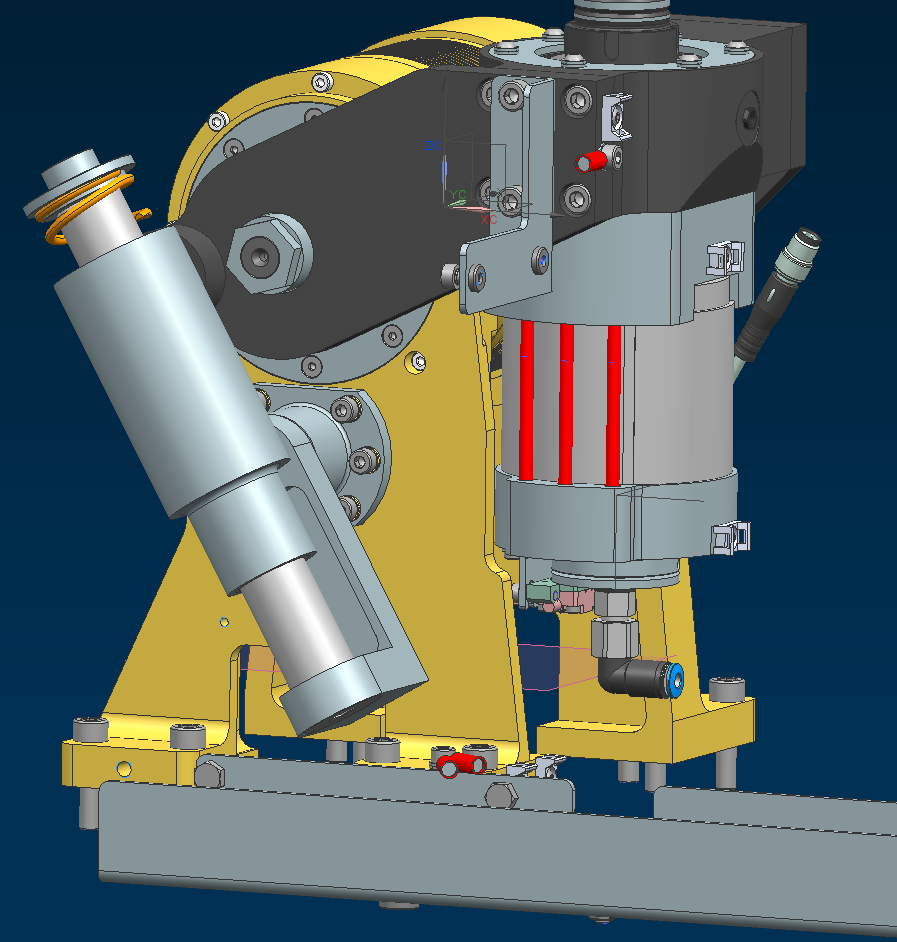
\includegraphics[width=0.5\linewidth]{./pics/rotXspring.png}
				\caption{Kompensationsfeder der RotX-Achse}
				\label{fig:rotXspring}
			\end{figure} 
			Diese Feder wird in der Simulation ebenfalls berücksichtigt und erzielt in der Simulation das gewünschte Verhalten. In Abbildung \ref{fig:M_rotXspring} ist der benötigte Momentenverlauf, welcher der Motor der RotX-Achse liefern muss, gezeigt.
			\begin{figure}[!h]
				\centering
				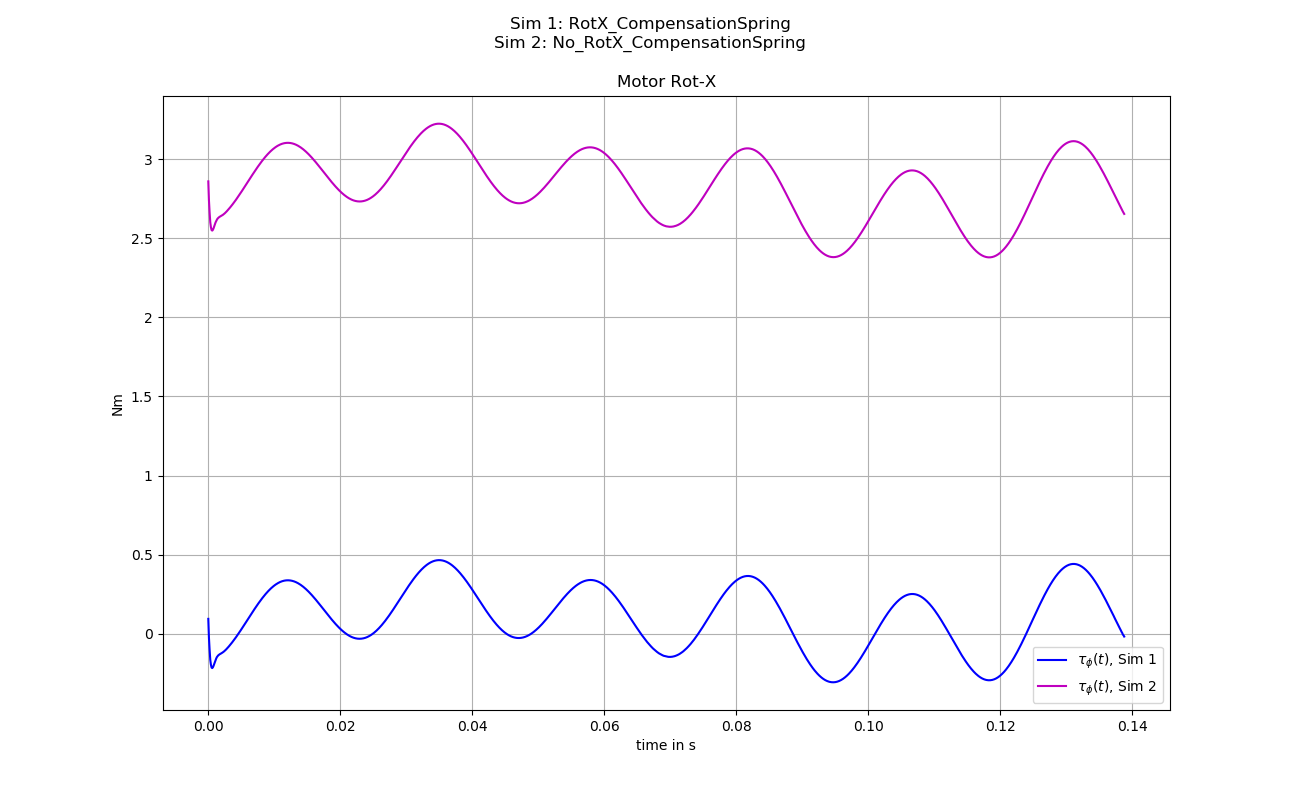
\includegraphics[width=0.99\linewidth]{./pics/M_rotXspring.png}
				\caption{Benötigter Momentenverlauf des Motors der RotX-Achse; Simulation ohne Kompensationsfeder (pink), Simulation mit Kompensationsfeder (blau)}
				\label{fig:M_rotXspring}
			\end{figure} 
			Diese Simulation stellt den \glqq worst case\grqq\text{ } bei einer Auslenkung von $ \varphi=0^{\circ} $ mit maximalem Moment durch das Eigengewicht dar.
			Die Eigenfrequenz dieser Feder mit den Parametern aus Abschnitt \ref{sec:modellparameter} wurde durch eine Simulation mit $ f_{0} = 1.35Hz $ identifiziert. Die zugehörige Steifigkeit der Druckfeder beträgt $ 1.895 \frac{N}{mm} $. Da die effektive Länge dieser Feder und somit die resultierende Kraft direkt vom Winkel $ \varphi $ abhängt, musste in der Simulationsumgebung kein weiterer Freiheitsgrad eingeführt werden. Stattdessen findet eine Umrechnung vom Winkel $ \varphi $ auf die effektive Federlänge statt. Damit ergibt sich das durch die Feder verursachte Kompensationsmoment um die RotX-Achse.
			
		\subsection{Modellierung der Antriebe}
			Die Motordynamik spielt ebenfalls eine Rolle bei der Modellierung eines Gesamtsystems. In diesem Abschnitt wird beschrieben wie die Motormodelle mit in die Simulation aufgenommen wurden. Vom Motorprinzip her handelt es sich bei allen drei Antrieben um 3-phasige permanenterregte Synchronmaschinen. Die beiden Linearachsen $ y $ und $ z $ sind spindelgetriebene indirekte Linearantriebe, die eine Berücksichtigung der Übersetzung erfordern. Die RotX-Achse wird durch einen Torque-Motor direkt angetrieben. Die Wicklungen aller drei Maschinen werden gemäß einem (einphasigen) Ersatzschaltbild einer PMSM \ref{fig:pmsm} berücksichtigt.  
			\begin{figure}[!h]
				\centering
				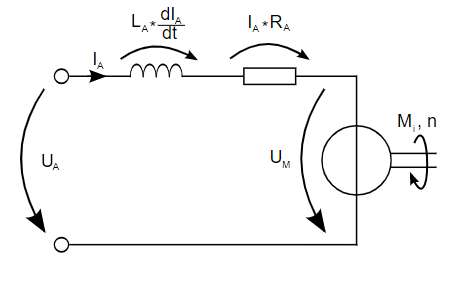
\includegraphics[width=0.4\linewidth]{./pics/pmsm.png}
				\caption{Prinzipschaltbild der Wicklungen einer PMSM}
				\label{fig:pmsm}
			\end{figure}
			Die zugehörige Zustandsdifferentialgleichung mit der Zwischenkreisspannung $ v_{A} $ als Eingangsgröße und dem Ankerstrom $ i_{A} $ als Zustandsgröße lautet somit für alle Antriebe
			\begin{align*}
				\frac{d i_{A}(t)}{dt} = \frac{1}{L}\bigg(v_{A}-i_{A}(t)R - k_{bemf}\cdot\omega_{M} \bigg).
			\end{align*}
			Die Berechnung der Winkelgeschwindigkeit ist, wie bereits erwähnt, von den Spindelsteigungen $ S_{y,z} $ abhängig und wird durch 
			\begin{align*}
				\omega_{y} &=\dfrac{ 2\pi \dot{y}}{S_{y}},  \qquad \omega_{z} =\dfrac{ 2\pi \dot{z}}{S_{z}}  
			\end{align*}
			berechnet.
			
			\subsubsection{Elektrische Parameter}
				\begin{tabular}{lp{1cm}p{8.6cm}}
					$ R_{y}= 1.5 \Omega$ && \textit{Ohmscher Ankerwiderstand des y-Motors}\\
					$ L_{y}= 2.7mH$ &&\textit{Induktivität der Ankerwicklung des y-Motors} \\ 
					$ k_{bemf,y}= 0.306 V/(rad/s)$ &&\textit{Back-EMF Konstante des y-Motors} \\ 
					$ \omega_{y} $ &&\textit{Winkelgeschwindigkeit des y-Motors} \\ 
					$ S_{y} $ &&\textit{Spindelsteigung des y-Motors} \\ 
					$ R_{z}= 0.6125\Omega$ && \textit{Ohmscher Ankerwiderstand des z-Motors}\\
					$ L_{z}= 5.0mH$ &&\textit{Induktivität der Ankerwicklung des z-Motors} \\ 
					$ k_{bemf,z}= 1.14 V/(rad/s)$ &&\textit{Back-EMF Konstante des z-Motors} \\ 
					$ \omega_{z}$ &&\textit{Winkelgeschwindigkeit des z-Motors} \\
					$ S_{z} $ &&\textit{Spindelsteigung des z-Motors} \\  
					$ R_{x}= 1.11\Omega$ && \textit{Ohmscher Ankerwiderstand des RotX-Motors}\\
					$ L_{x}= 3.4mH$ &&\textit{Induktivität der Ankerwicklung des RotX-Motors} \\ 
					$ k_{bemf,x}= 0.266 V/(rad/s)$ &&\textit{Back-EMF Konstante des RotX-Motors} \\ 
					$ \omega_{x} $ &&\textit{Winkelgeschwindigkeit des RotX-Motors} \\ 
				\end{tabular}\leavevmode\\
			
			\subsubsection{Struktur des gesamten Regelkreises}
				Die gesamte Regelkreisstruktur setzt sich aus einem Äußeren Regelkreis und einem unterlagerten Stromregelkreis der einzelnen Achsen zusammen (siehe Abbildung \ref{fig:Regelkreis}). Das Prinzip des äußeren Regelkreises nennt sich \textit{computed-torque feedback}. Dabei wird die Fehlerdynamik des mechanischen Systems durch Einführung eines neuen Eingangs
				\[ \bm{v}= \ddot{\bm{q}}_{ref} - K_{1}\underbrace{(\dot{\bm{q}} - \dot{\bm{q}}_{ref})}_{\dot{\bm{e}}_{q}}- K_{0}\underbrace{(\bm{q} - \bm{q}_{ref})}_{\bm{e}_{q}} \] 
				linearisiert. Die benötigten Gelenkskräfte/-momente können dann über das inverse Modell gemäß
				\[ \bm{\tau} =  M\bm{v} + C\dot{\bm{q}} - F\]
				berechnet werden. Der große Vorteil dabei ist, dass eine lineare Fehlerdynamik für das nichtlineare System angewendet werden kann.
				\begin{figure}[!h]
					\centering
					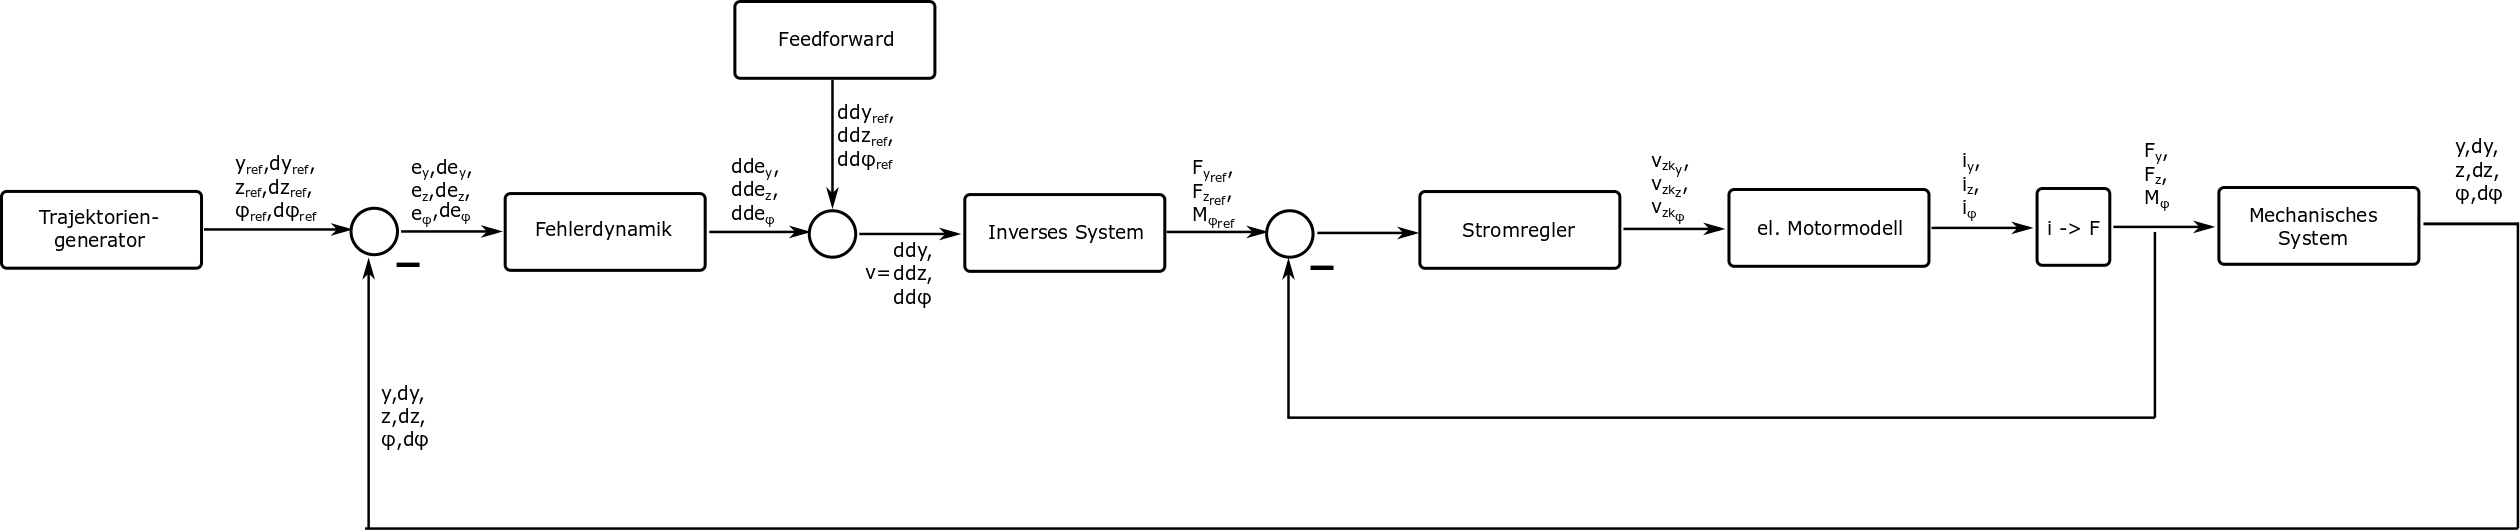
\includegraphics[width=0.99\linewidth]{./pics/Regelstruktur.png}
					\caption{Gesamte Regelkreisstruktur mit $ \bm{\tau}_{ref} = [F_{y_{ref}},F_{z_{ref}},M_{\varphi_{ref}}]^{T} $, $ \bm{\tau} = [F_{y},F_{z},M_{\varphi}]^{T} $,  $ \bm{q} = [y,z,\varphi]^{T} $, $ \bm{q}_{ref} = [y_{ref},z_{ref},\varphi_{ref}]^{T} $, $ \bm{e}_{q} = [e_{y},e_{y},e_{\varphi}]^{T} $} und den zugehörigen Ableitung der jeweiligen Vektoren
					\label{fig:Regelkreis}
				\end{figure}
				Diesem \textit{computed-torque} Regelkreis ist der elektrische Stromregelkreis mit den oben beschriebenen Motormodellen unterlagert.
	\clearpage	
	\section{Parametrierung und Modellabgleich (AP 2.2)}
%	
%\section{Entwicklung von erweiterten Regelungskonzepten (AP 3)}
%\section{Umsetzung und Test der Regelungskonzepte (AP 4)}
%	\subsection{Umsetzung der Regelungskonzepte (AP 4.1)}
%	\subsection{Validierung und Bewertung der erweiterten Regelungskonzepte an der realen Hardware (AP 4.2)}
\end{document}